\documentclass{article}
\renewcommand{\thesection}{\Roman{section}}
% \renewcommand{\thesubsection}{\thesection.\Roman{subsection}}
\usepackage{amsmath}
\usepackage{helvet}
\usepackage{graphbox}
\usepackage{subcaption}
\usepackage{blindtext}
\usepackage{parskip}
\usepackage{multicol}
\usepackage{graphicx}
\graphicspath{ {./resources/photos/} }
\setlength{\columnsep}{1cm}
\title{
  % Simulation of misinformation spreading processes
  % in social networks: an application with NetLogo

  Notes
}
\author{Elizer F. Dolorosa}
\date{May 2024}

\begin{document}
\maketitle

\section{CONCEPT}
SBFC Model \textbf{BUT} with the concept of "friend groups" introduced. The idea essentially is that a person's friend group, that leans on either believing or not in a news, could influence their "SBFC" state.

\begin{figure}[h]
  \begin{subfigure}{0.57\textwidth}
    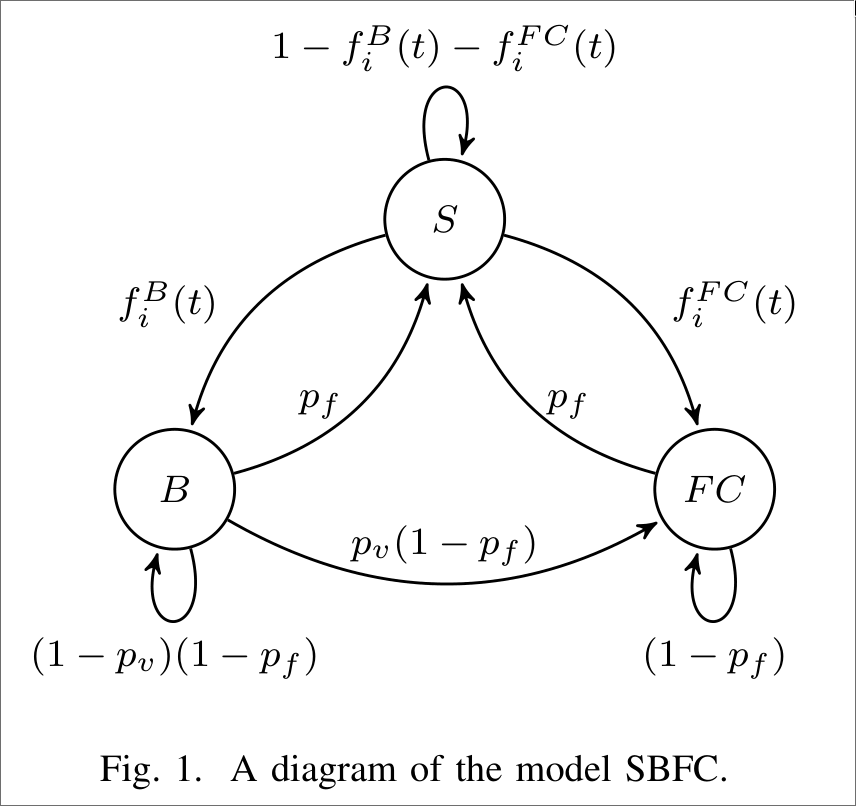
\includegraphics[align=c,width=6.9cm, height=7cm]{sbfc-diagram.png}
  \end{subfigure}
  \begin{subfigure}{0.42\textwidth}
    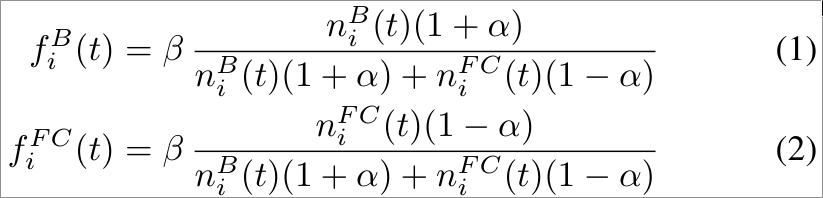
\includegraphics[align=c,width=5cm, height=1.5cm]{transmission-eq.png}
  \end{subfigure}
  % \centering
\end{figure}

% TODO: Write more about this on the paper.
Instead of devising a mechanism in creating groups, the Louvain
community detection algorithm is used. This algorithm, as described,
detects community or as we can call it "friend groups", which are
described to be dense in terms of connections in-community vs out-community.
This happens to be compatible with the Barabasi-Albert and the Erdos-Renyi
algorithm, which the study this was based on was using to generate networks.

Before we begin to assimilate the concept, we assume the following about the new concept:
\begin{enumerate}
  \item The "inherent bias" of communities stay the same all throughout the simulation;
  \item The amount of people in friend groups stays the same; and
  \item All agents are part of a group due to the nature of their
    Louvain community detection algorithm.
\end{enumerate}

\begin{sloppypar}
  As a result, the following parameters/variables are added
with some caveats/edge cases to consider:
\end{sloppypar}
\begin{enumerate}
  \item percentage of friend groups to be \textit{FC}'s
  \item percentage of community influence
\end{enumerate}

% With that being said, edge cases must be considered. For example,
% we should check if the percentage of the population to be in a friend
% group can allow more than one groups to form.
%
% If checking/restricting the input from slider is hard or impossible,
% we can resort to \textbf{failsafes} (if the aforementioned edge case occurs,
% allow only 1 group to form).

% \pagebreak
Let $h_i^{B|FC}$ return 1 if agent's friend group is $B|FC$ accordingly, otherwise 0. 

Let $c_i^G(t)$ return $i's$ \# of $G$ "friend" neighbors. Let $o_i^G(t)$ return $i's$ \# of $G$ "non-friend" neighbors. Let $\omega$ = group friends' influence to be a fact-checker such that $\omega \in [0,1]$. Thus:
% \[g_i^{B|FC} = h_i^{B|FC}g_i(1+\omega)\]

% Let $n_i^{B|FC}(t)$ = $B|FC$ neighbors of agent $i$ at time $t$
Let $n_i^{B|FC}(t)$ be the number $B|FC$ neighbors of agent $i$ at time $t$,
multiplied by their friends' influence if applicable:
\begin{equation} n_i^G(t)=m_i^G\,c_i^G(t)+o_i^G(t) \end{equation}
\begin{equation}
  m_i^G= 
  \begin{cases}
    1 + \omega & \text{if}\; h_i^G = 1 \\
    1 & \text{if}\; h_i^G = 0 \\
  \end{cases} \end{equation}
where $G$ is either \textit{B} or \textit{FC}

\begin{equation}
  p_i(t+1) = (p_i^S(t+1),p_i^B(t+1),p_i^{FC}(t+1))
\end{equation}
\begin{equation}
  p_i^S(t+1) = [1-f_i^B(t)-f_i^{FC}(t)]s_i(t)+p_f[s_i^B(t)+s_i^{FC}(t)]
\end{equation}
\begin{equation}
  p_i^B(t+1) = f_i^B(t)s_i^S(t) + (1-p_f)(1-p_v)s_i^B(t)
\end{equation}
\begin{equation}
  p_i^{FC}(t+1) = f_i^{FC}(t)s_i^S(t) + p_vs_i^B(t)+(1-p_f)s_i^{FC}(t)
\end{equation}

\begin{equation}
  s_i^{\{S,B,FC\}}(t)=\delta(s_i(t), \{S,B,FC\})
\end{equation}

And so the spreading transitions stay the same:

% TODO: verify math syntax
\begin{equation}f_i^B(t)=\beta\frac{n_i^B(t)(1+\alpha)}{n_i^B(t)(1+\alpha)+n_i^{FC}(t)(1-\alpha)}\end{equation}

\begin{equation}f_i^{FC}(t)=\beta\frac{n_i^{FC}(t)(1-\alpha)}{n_i^B(t)(1+\alpha)+n_i^{FC}(t)(1-\alpha)}\end{equation}

\textit{Verifying} transition should be affected by the
the agent's friend group somehow. We represent this as
the following:

\begin{equation} 
  % TODO: verify math "syntax"
  v_i = 
  \begin{cases} 
      1+\omega & \text{if}\ h_i^{FC} = 1 \\
      1-\omega & \text{if}\ h_i^B = 1 \\
  \end{cases}
\end{equation}
\begin{equation} p_i = v_i\;v_g \end{equation}

where $v_i$ is the old $p_v$ or the verifying probability

As for \textit{forgetting} transitions, I left it as it is.

\section{RESULTS}
Barabasi-Albert ($\alpha$ = 0.30): All in all, as $F_c$ increases, the less the "increase" of the believer group's population as $F_i$ increases is.

Barabasi-Albert ($\alpha$ = 0.80): As $F_c$ goes up, the less the "increase" of the believer group's population as $F_i$ increases is.
When $F_c = 0.75$,  the fact-checkers were able to outnumber the believer groups.

Erdos-Renyi ($\alpha$ = 0.30): All in all, as $F_c$ increases, the less the "increase" of the believer group's population as $F_i$ increases is.

Erdos-Renyi ($\alpha$ = 0.80): As $F_c$ goes up, the less the "increase" of the believer group's population as $F_i$ increases is
When $F_c = 0.75$,  the fact-checkers were able to outnumber the believer groups.

% \begin{multicols*}{2}
%
% \section{FIRST SECTION}
% All human things are subject to decay. And when fate summons, Monarchs must obey.
%
% \section{METHODOLOGY}
% All human things are subject to decay. And when fate summons, Monarchs must obey.
%
% \section{RESULTS AND DISCUSSIONS}
% All human things are subject to decay. And when fate summons, Monarchs must obey.
%
% \section{CONCLUSION}
% All human things are subject to decay. And when fate summons, Monarchs must obey.
%
% % \blindtext\blindtext
% \end{multicols*}

\end{document}
